% SmartCom 2027 (Springer LNNS) version -- GENERATED by make_smartcom.py from bpp_v3_conf.tex; edit that file, then rerun.
\documentclass{svproc}
\usepackage{amsmath,amssymb}
\usepackage{graphicx}
\usepackage{booktabs}
\usepackage{array}
\usepackage{xspace}
\usepackage[table]{xcolor}
% numbered citations in square brackets, sorted and compressed ([3, 5-7]); Springer's LaTeX instructions call
% numbered citation "preferred" and the list "ideally sorted in alphabetical order": spmpsci.bst (MathPhySci) does both
\usepackage[numbers,sort&compress]{natbib}
% svproc defines \chapter, so natbib would start the references with \chapter* on a new page in normal size;
% use svproc's own reference layout instead: an unnumbered section in \small, entries labeled "1."
\renewcommand{\bibsection}{\section*{References}}
\renewcommand{\bibfont}{\small}
\renewcommand{\bibnumfmt}[1]{#1.}
\usepackage{float}
\usepackage{capt-of}
\usepackage{flafter}  % a float never appears before the text that defines it (keeps Table 2 below the Method heading)
\usepackage{xurl}
\def\UrlFont{\rmfamily}
\usepackage[hidelinks]{hyperref}  % clickable cross-references and citations (Springer: \label/\ref become links)
\graphicspath{{figures/}}
\hyphenation{Table Tables Figure Figures ri-san-ki-zu-mab up-a-da-ci-ti-nib gu-sel-ku-mab ra-vu-li-zu-mab
  ro-za-no-li-xi-zu-mab el-a-fi-bra-nor us-te-ki-nu-mab am-i-fam-pri-dine}
\newcommand{\sysname}{BioPathNet++\xspace}
\newcommand{\MainValidMrr}{0.394}
\newcommand{\MainValidMrrSd}{0.003}
\newcommand{\MainValidHitsOne}{0.353}
\newcommand{\MainValidHitsOneSd}{0.008}
\newcommand{\MainValidHitsTen}{0.456}
\newcommand{\MainValidHitsTenSd}{0.018}
\newcommand{\MainValidHitsHundred}{0.669}
\newcommand{\MainValidHitsHundredSd}{0.021}
\newcommand{\MainValidAuroc}{0.938}
\newcommand{\MainValidAurocSd}{0.001}
\newcommand{\MainValidAuprc}{0.424}
\newcommand{\MainValidAuprcSd}{0.005}
\newcommand{\MainValidAurocHard}{0.799}
\newcommand{\MainValidAurocHardSd}{0.010}
\newcommand{\MainValidAurocDeg}{0.886}
\newcommand{\MainValidAurocDegSd}{0.010}
\newcommand{\MainValidAnyTen}{56}
\newcommand{\MainTargetsMrr}{0.475}
\newcommand{\MainTargetsMrrSd}{0.017}
\newcommand{\MainTargetsHitsOne}{0.396}
\newcommand{\MainTargetsHitsOneSd}{0.038}
\newcommand{\MainTargetsHitsTen}{0.648}
\newcommand{\MainTargetsHitsTenSd}{0.033}
\newcommand{\MainTargetsHitsHundred}{0.716}
\newcommand{\MainTargetsHitsHundredSd}{0.016}
\newcommand{\MainTargetsAuroc}{0.982}
\newcommand{\MainTargetsAurocSd}{0.008}
\newcommand{\MainTargetsAuprc}{0.594}
\newcommand{\MainTargetsAuprcSd}{0.010}
\newcommand{\MainTargetsAurocHard}{0.892}
\newcommand{\MainTargetsAurocHardSd}{0.020}
\newcommand{\MainTargetsAurocDeg}{0.954}
\newcommand{\MainTargetsAurocDegSd}{0.031}
\newcommand{\MainTargetsAnyTen}{83}
\newcommand{\MainSeeds}{3}
\newcommand{\PathsValidMrr}{0.405}
\newcommand{\PathsValidMrrSd}{0.013}
\newcommand{\PathsValidHitsOne}{0.363}
\newcommand{\PathsValidHitsOneSd}{0.019}
\newcommand{\PathsValidHitsTen}{0.479}
\newcommand{\PathsValidHitsTenSd}{0.025}
\newcommand{\PathsValidHitsHundred}{0.663}
\newcommand{\PathsValidHitsHundredSd}{0.018}
\newcommand{\PathsValidAuroc}{0.946}
\newcommand{\PathsValidAurocSd}{0.004}
\newcommand{\PathsValidAuprc}{0.443}
\newcommand{\PathsValidAuprcSd}{0.010}
\newcommand{\PathsValidAurocHard}{0.829}
\newcommand{\PathsValidAurocHardSd}{0.011}
\newcommand{\PathsValidAurocDeg}{0.888}
\newcommand{\PathsValidAurocDegSd}{0.009}
\newcommand{\PathsValidAnyTen}{59}
\newcommand{\PathsTargetsMrr}{0.463}
\newcommand{\PathsTargetsMrrSd}{0.087}
\newcommand{\PathsTargetsHitsOne}{0.375}
\newcommand{\PathsTargetsHitsOneSd}{0.134}
\newcommand{\PathsTargetsHitsTen}{0.657}
\newcommand{\PathsTargetsHitsTenSd}{0.025}
\newcommand{\PathsTargetsHitsHundred}{0.738}
\newcommand{\PathsTargetsHitsHundredSd}{0.023}
\newcommand{\PathsTargetsAuroc}{0.986}
\newcommand{\PathsTargetsAurocSd}{0.004}
\newcommand{\PathsTargetsAuprc}{0.577}
\newcommand{\PathsTargetsAuprcSd}{0.054}
\newcommand{\PathsTargetsAurocHard}{0.907}
\newcommand{\PathsTargetsAurocHardSd}{0.007}
\newcommand{\PathsTargetsAurocDeg}{0.968}
\newcommand{\PathsTargetsAurocDegSd}{0.015}
\newcommand{\PathsTargetsAnyTen}{83}
\newcommand{\PathsSeeds}{3}
\newcommand{\PriorValidMrr}{0.306}
\newcommand{\PriorValidMrrSd}{0.003}
\newcommand{\PriorValidHitsOne}{0.268}
\newcommand{\PriorValidHitsOneSd}{0.004}
\newcommand{\PriorValidHitsTen}{0.354}
\newcommand{\PriorValidHitsTenSd}{0.006}
\newcommand{\PriorValidHitsHundred}{0.531}
\newcommand{\PriorValidHitsHundredSd}{0.008}
\newcommand{\PriorValidAuroc}{0.885}
\newcommand{\PriorValidAurocSd}{0.002}
\newcommand{\PriorValidAuprc}{0.335}
\newcommand{\PriorValidAuprcSd}{0.003}
\newcommand{\PriorValidAurocHard}{0.700}
\newcommand{\PriorValidAurocHardSd}{0.013}
\newcommand{\PriorValidAurocDeg}{0.844}
\newcommand{\PriorValidAurocDegSd}{0.001}
\newcommand{\PriorValidAnyTen}{46}
\newcommand{\PriorTargetsMrr}{0.330}
\newcommand{\PriorTargetsMrrSd}{0.025}
\newcommand{\PriorTargetsHitsOne}{0.263}
\newcommand{\PriorTargetsHitsOneSd}{0.034}
\newcommand{\PriorTargetsHitsTen}{0.490}
\newcommand{\PriorTargetsHitsTenSd}{0.007}
\newcommand{\PriorTargetsHitsHundred}{0.720}
\newcommand{\PriorTargetsHitsHundredSd}{0.004}
\newcommand{\PriorTargetsAuroc}{0.956}
\newcommand{\PriorTargetsAurocSd}{0.000}
\newcommand{\PriorTargetsAuprc}{0.447}
\newcommand{\PriorTargetsAuprcSd}{0.028}
\newcommand{\PriorTargetsAurocHard}{0.780}
\newcommand{\PriorTargetsAurocHardSd}{0.002}
\newcommand{\PriorTargetsAurocDeg}{0.910}
\newcommand{\PriorTargetsAurocDegSd}{0.001}
\newcommand{\PriorTargetsAnyTen}{83}
\newcommand{\PriorSeeds}{3}
\newcommand{\NoautoValidMrr}{0.445}
\newcommand{\NoautoValidMrrSd}{0.008}
\newcommand{\NoautoValidHitsOne}{0.387}
\newcommand{\NoautoValidHitsOneSd}{0.011}
\newcommand{\NoautoValidHitsTen}{0.554}
\newcommand{\NoautoValidHitsTenSd}{0.005}
\newcommand{\NoautoValidHitsHundred}{0.719}
\newcommand{\NoautoValidHitsHundredSd}{0.004}
\newcommand{\NoautoValidAuroc}{0.949}
\newcommand{\NoautoValidAurocSd}{0.004}
\newcommand{\NoautoValidAuprc}{0.482}
\newcommand{\NoautoValidAuprcSd}{0.006}
\newcommand{\NoautoValidAurocHard}{0.840}
\newcommand{\NoautoValidAurocHardSd}{0.003}
\newcommand{\NoautoValidAurocDeg}{0.901}
\newcommand{\NoautoValidAurocDegSd}{0.009}
\newcommand{\NoautoValidAnyTen}{70}
\newcommand{\NoautoTargetsMrr}{0.487}
\newcommand{\NoautoTargetsMrrSd}{0.031}
\newcommand{\NoautoTargetsHitsOne}{0.409}
\newcommand{\NoautoTargetsHitsOneSd}{0.037}
\newcommand{\NoautoTargetsHitsTen}{0.615}
\newcommand{\NoautoTargetsHitsTenSd}{0.022}
\newcommand{\NoautoTargetsHitsHundred}{0.736}
\newcommand{\NoautoTargetsHitsHundredSd}{0.037}
\newcommand{\NoautoTargetsAuroc}{0.981}
\newcommand{\NoautoTargetsAurocSd}{0.006}
\newcommand{\NoautoTargetsAuprc}{0.592}
\newcommand{\NoautoTargetsAuprcSd}{0.024}
\newcommand{\NoautoTargetsAurocHard}{0.904}
\newcommand{\NoautoTargetsAurocHardSd}{0.018}
\newcommand{\NoautoTargetsAurocDeg}{0.939}
\newcommand{\NoautoTargetsAurocDegSd}{0.022}
\newcommand{\NoautoTargetsAnyTen}{83}
\newcommand{\NoautoAreaMrr}{0.449}
\newcommand{\NoautoAreaMrrSd}{0.042}
\newcommand{\NoautoAreaHitsOne}{0.355}
\newcommand{\NoautoAreaHitsOneSd}{0.054}
\newcommand{\NoautoAreaHitsTen}{0.640}
\newcommand{\NoautoAreaHitsTenSd}{0.037}
\newcommand{\NoautoAreaHitsHundred}{0.730}
\newcommand{\NoautoAreaHitsHundredSd}{0.011}
\newcommand{\NoautoAreaAuroc}{0.951}
\newcommand{\NoautoAreaAurocSd}{0.004}
\newcommand{\NoautoAreaAuprc}{0.507}
\newcommand{\NoautoAreaAuprcSd}{0.030}
\newcommand{\NoautoAreaAurocHard}{0.819}
\newcommand{\NoautoAreaAurocHardSd}{0.008}
\newcommand{\NoautoAreaAurocDeg}{0.922}
\newcommand{\NoautoAreaAurocDegSd}{0.015}
\newcommand{\NoautoAreaAnyTen}{76}
\newcommand{\NoautoSeeds}{3}
\newcommand{\NoautoPathsValidMrr}{0.445}
\newcommand{\NoautoPathsValidMrrSd}{0.006}
\newcommand{\NoautoPathsValidHitsOne}{0.378}
\newcommand{\NoautoPathsValidHitsOneSd}{0.006}
\newcommand{\NoautoPathsValidHitsTen}{0.546}
\newcommand{\NoautoPathsValidHitsTenSd}{0.006}
\newcommand{\NoautoPathsValidHitsHundred}{0.721}
\newcommand{\NoautoPathsValidHitsHundredSd}{0.002}
\newcommand{\NoautoPathsValidAuroc}{0.951}
\newcommand{\NoautoPathsValidAurocSd}{0.005}
\newcommand{\NoautoPathsValidAuprc}{0.486}
\newcommand{\NoautoPathsValidAuprcSd}{0.006}
\newcommand{\NoautoPathsValidAurocHard}{0.849}
\newcommand{\NoautoPathsValidAurocHardSd}{0.010}
\newcommand{\NoautoPathsValidAurocDeg}{0.915}
\newcommand{\NoautoPathsValidAurocDegSd}{0.007}
\newcommand{\NoautoPathsValidAnyTen}{69}
\newcommand{\NoautoPathsTargetsMrr}{0.520}
\newcommand{\NoautoPathsTargetsMrrSd}{0.036}
\newcommand{\NoautoPathsTargetsHitsOne}{0.460}
\newcommand{\NoautoPathsTargetsHitsOneSd}{0.055}
\newcommand{\NoautoPathsTargetsHitsTen}{0.638}
\newcommand{\NoautoPathsTargetsHitsTenSd}{0.006}
\newcommand{\NoautoPathsTargetsHitsHundred}{0.747}
\newcommand{\NoautoPathsTargetsHitsHundredSd}{0.004}
\newcommand{\NoautoPathsTargetsAuroc}{0.975}
\newcommand{\NoautoPathsTargetsAurocSd}{0.002}
\newcommand{\NoautoPathsTargetsAuprc}{0.607}
\newcommand{\NoautoPathsTargetsAuprcSd}{0.012}
\newcommand{\NoautoPathsTargetsAurocHard}{0.894}
\newcommand{\NoautoPathsTargetsAurocHardSd}{0.005}
\newcommand{\NoautoPathsTargetsAurocDeg}{0.906}
\newcommand{\NoautoPathsTargetsAurocDegSd}{0.019}
\newcommand{\NoautoPathsTargetsAnyTen}{83}
\newcommand{\NoautoPathsAreaMrr}{0.416}
\newcommand{\NoautoPathsAreaMrrSd}{0.037}
\newcommand{\NoautoPathsAreaHitsOne}{0.284}
\newcommand{\NoautoPathsAreaHitsOneSd}{0.061}
\newcommand{\NoautoPathsAreaHitsTen}{0.621}
\newcommand{\NoautoPathsAreaHitsTenSd}{0.009}
\newcommand{\NoautoPathsAreaHitsHundred}{0.734}
\newcommand{\NoautoPathsAreaHitsHundredSd}{0.002}
\newcommand{\NoautoPathsAreaAuroc}{0.947}
\newcommand{\NoautoPathsAreaAurocSd}{0.004}
\newcommand{\NoautoPathsAreaAuprc}{0.491}
\newcommand{\NoautoPathsAreaAuprcSd}{0.018}
\newcommand{\NoautoPathsAreaAurocHard}{0.818}
\newcommand{\NoautoPathsAreaAurocHardSd}{0.009}
\newcommand{\NoautoPathsAreaAurocDeg}{0.937}
\newcommand{\NoautoPathsAreaAurocDegSd}{0.006}
\newcommand{\NoautoPathsAreaAnyTen}{71}
\newcommand{\NoautoPathsSeeds}{3}
\newcommand{\BrgValidMrr}{0.404}
\newcommand{\BrgValidMrrSd}{0.006}
\newcommand{\BrgValidHitsOne}{0.350}
\newcommand{\BrgValidHitsOneSd}{0.007}
\newcommand{\BrgValidHitsTen}{0.492}
\newcommand{\BrgValidHitsTenSd}{0.004}
\newcommand{\BrgValidHitsHundred}{0.700}
\newcommand{\BrgValidHitsHundredSd}{0.011}
\newcommand{\BrgValidAuroc}{0.947}
\newcommand{\BrgValidAurocSd}{0.005}
\newcommand{\BrgValidAuprc}{0.438}
\newcommand{\BrgValidAuprcSd}{0.005}
\newcommand{\BrgValidAurocHard}{0.831}
\newcommand{\BrgValidAurocHardSd}{0.020}
\newcommand{\BrgValidAurocDeg}{0.904}
\newcommand{\BrgValidAurocDegSd}{0.006}
\newcommand{\BrgValidAnyTen}{61}
\newcommand{\BrgTargetsMrr}{0.504}
\newcommand{\BrgTargetsMrrSd}{0.075}
\newcommand{\BrgTargetsHitsOne}{0.426}
\newcommand{\BrgTargetsHitsOneSd}{0.121}
\newcommand{\BrgTargetsHitsTen}{0.657}
\newcommand{\BrgTargetsHitsTenSd}{0.021}
\newcommand{\BrgTargetsHitsHundred}{0.771}
\newcommand{\BrgTargetsHitsHundredSd}{0.024}
\newcommand{\BrgTargetsAuroc}{0.990}
\newcommand{\BrgTargetsAurocSd}{0.001}
\newcommand{\BrgTargetsAuprc}{0.609}
\newcommand{\BrgTargetsAuprcSd}{0.038}
\newcommand{\BrgTargetsAurocHard}{0.913}
\newcommand{\BrgTargetsAurocHardSd}{0.010}
\newcommand{\BrgTargetsAurocDeg}{0.983}
\newcommand{\BrgTargetsAurocDegSd}{0.017}
\newcommand{\BrgTargetsAnyTen}{83}
\newcommand{\BrgSeeds}{3}
\newcommand{\BceValidMrr}{0.378}
\newcommand{\BceValidMrrSd}{0.028}
\newcommand{\BceValidHitsOne}{0.339}
\newcommand{\BceValidHitsOneSd}{0.036}
\newcommand{\BceValidHitsTen}{0.452}
\newcommand{\BceValidHitsTenSd}{0.017}
\newcommand{\BceValidHitsHundred}{0.652}
\newcommand{\BceValidHitsHundredSd}{0.031}
\newcommand{\BceValidAuroc}{0.942}
\newcommand{\BceValidAurocSd}{0.015}
\newcommand{\BceValidAuprc}{0.411}
\newcommand{\BceValidAuprcSd}{0.020}
\newcommand{\BceValidAurocHard}{0.815}
\newcommand{\BceValidAurocHardSd}{0.061}
\newcommand{\BceValidAurocDeg}{0.887}
\newcommand{\BceValidAurocDegSd}{0.018}
\newcommand{\BceValidAnyTen}{55}
\newcommand{\BceTargetsMrr}{0.320}
\newcommand{\BceTargetsMrrSd}{0.046}
\newcommand{\BceTargetsHitsOne}{0.239}
\newcommand{\BceTargetsHitsOneSd}{0.034}
\newcommand{\BceTargetsHitsTen}{0.540}
\newcommand{\BceTargetsHitsTenSd}{0.095}
\newcommand{\BceTargetsHitsHundred}{0.695}
\newcommand{\BceTargetsHitsHundredSd}{0.008}
\newcommand{\BceTargetsAuroc}{0.982}
\newcommand{\BceTargetsAurocSd}{0.003}
\newcommand{\BceTargetsAuprc}{0.441}
\newcommand{\BceTargetsAuprcSd}{0.059}
\newcommand{\BceTargetsAurocHard}{0.880}
\newcommand{\BceTargetsAurocHardSd}{0.018}
\newcommand{\BceTargetsAurocDeg}{0.926}
\newcommand{\BceTargetsAurocDegSd}{0.035}
\newcommand{\BceTargetsAnyTen}{83}
\newcommand{\BceSeeds}{3}
\newcommand{\KnnValidMrr}{0.281}
\newcommand{\KnnValidHitsTen}{0.350}
\newcommand{\KnnValidAuroc}{0.860}
\newcommand{\KnnValidAurocHard}{0.661}
\newcommand{\KnnValidAnyTen}{44}
\newcommand{\KnnTargetsMrr}{0.296}
\newcommand{\KnnTargetsHitsTen}{0.424}
\newcommand{\KnnTargetsAuroc}{0.962}
\newcommand{\KnnTargetsAurocHard}{0.778}
\newcommand{\KnnTargetsAnyTen}{67}
\newcommand{\PopValidMrr}{0.046}
\newcommand{\PopValidHitsTen}{0.049}
\newcommand{\PopValidAuroc}{0.830}
\newcommand{\PopValidAurocHard}{0.476}
\newcommand{\PopValidAnyTen}{15}
\newcommand{\PopTargetsMrr}{0.099}
\newcommand{\PopTargetsHitsTen}{0.148}
\newcommand{\PopTargetsAuroc}{0.905}
\newcommand{\PopTargetsAurocHard}{0.460}
\newcommand{\PopTargetsAnyTen}{50}
\newcommand{\RandValidMrr}{0.001}
\newcommand{\RandValidHitsTen}{0.002}
\newcommand{\RandValidAuroc}{0.471}
\newcommand{\RandValidAurocHard}{0.488}
\newcommand{\RandValidAnyTen}{1}
\newcommand{\RandTargetsMrr}{0.001}
\newcommand{\RandTargetsHitsTen}{0.000}
\newcommand{\RandTargetsAuroc}{0.476}
\newcommand{\RandTargetsAurocHard}{0.488}
\newcommand{\RandTargetsAnyTen}{0}
\newcommand{\DegValidMrr}{0.004}
\newcommand{\DegValidHitsTen}{0.003}
\newcommand{\DegValidAuroc}{0.783}
\newcommand{\DegValidAurocHard}{0.421}
\newcommand{\DegValidAnyTen}{1}
\newcommand{\DegTargetsMrr}{0.003}
\newcommand{\DegTargetsHitsTen}{0.000}
\newcommand{\DegTargetsAuroc}{0.732}
\newcommand{\DegTargetsAurocHard}{0.404}
\newcommand{\DegTargetsAnyTen}{0}
\newcommand{\NoautoKnnValidMrr}{0.347}
\newcommand{\NoautoKnnValidHitsTen}{0.407}
\newcommand{\NoautoKnnValidAuroc}{0.890}
\newcommand{\NoautoKnnValidAurocHard}{0.748}
\newcommand{\NoautoKnnValidAnyTen}{53}
\newcommand{\NoautoKnnTargetsMrr}{0.273}
\newcommand{\NoautoKnnTargetsHitsTen}{0.594}
\newcommand{\NoautoKnnTargetsAuroc}{0.857}
\newcommand{\NoautoKnnTargetsAurocHard}{0.790}
\newcommand{\NoautoKnnTargetsAnyTen}{83}
\newcommand{\NoautoKnnAreaMrr}{0.311}
\newcommand{\NoautoKnnAreaHitsTen}{0.469}
\newcommand{\NoautoKnnAreaAuroc}{0.832}
\newcommand{\NoautoKnnAreaAurocHard}{0.712}
\newcommand{\NoautoKnnAreaAnyTen}{57}
\newcommand{\NoautoPopValidMrr}{0.054}
\newcommand{\NoautoPopValidHitsTen}{0.054}
\newcommand{\NoautoPopValidAuroc}{0.871}
\newcommand{\NoautoPopValidAurocHard}{0.639}
\newcommand{\NoautoPopValidAnyTen}{12}
\newcommand{\NoautoPopTargetsMrr}{0.093}
\newcommand{\NoautoPopTargetsHitsTen}{0.148}
\newcommand{\NoautoPopTargetsAuroc}{0.799}
\newcommand{\NoautoPopTargetsAurocHard}{0.519}
\newcommand{\NoautoPopTargetsAnyTen}{50}
\newcommand{\NoautoPopAreaMrr}{0.260}
\newcommand{\NoautoPopAreaHitsTen}{0.346}
\newcommand{\NoautoPopAreaAuroc}{0.808}
\newcommand{\NoautoPopAreaAurocHard}{0.604}
\newcommand{\NoautoPopAreaAnyTen}{48}
\newcommand{\NoautoRandValidMrr}{0.001}
\newcommand{\NoautoRandValidHitsTen}{0.005}
\newcommand{\NoautoRandValidAuroc}{0.428}
\newcommand{\NoautoRandValidAurocHard}{0.443}
\newcommand{\NoautoRandValidAnyTen}{2}
\newcommand{\NoautoRandTargetsMrr}{0.001}
\newcommand{\NoautoRandTargetsHitsTen}{0.000}
\newcommand{\NoautoRandTargetsAuroc}{0.476}
\newcommand{\NoautoRandTargetsAurocHard}{0.488}
\newcommand{\NoautoRandTargetsAnyTen}{0}
\newcommand{\NoautoRandAreaMrr}{0.000}
\newcommand{\NoautoRandAreaHitsTen}{0.000}
\newcommand{\NoautoRandAreaAuroc}{0.419}
\newcommand{\NoautoRandAreaAurocHard}{0.436}
\newcommand{\NoautoRandAreaAnyTen}{0}
\newcommand{\NoautoDegValidMrr}{0.003}
\newcommand{\NoautoDegValidHitsTen}{0.001}
\newcommand{\NoautoDegValidAuroc}{0.778}
\newcommand{\NoautoDegValidAurocHard}{0.435}
\newcommand{\NoautoDegValidAnyTen}{2}
\newcommand{\NoautoDegTargetsMrr}{0.003}
\newcommand{\NoautoDegTargetsHitsTen}{0.000}
\newcommand{\NoautoDegTargetsAuroc}{0.732}
\newcommand{\NoautoDegTargetsAurocHard}{0.404}
\newcommand{\NoautoDegTargetsAnyTen}{0}
\newcommand{\NoautoDegAreaMrr}{0.003}
\newcommand{\NoautoDegAreaHitsTen}{0.000}
\newcommand{\NoautoDegAreaAuroc}{0.820}
\newcommand{\NoautoDegAreaAurocHard}{0.443}
\newcommand{\NoautoDegAreaAnyTen}{0}
\newcommand{\DiffMainKnnValid}{+0.113}
\newcommand{\PbootMainKnnValid}{$<$0.001}
\newcommand{\PwilMainKnnValid}{$<$0.001}
\newcommand{\DiffLoMainKnnValid}{+0.056}
\newcommand{\DiffHiMainKnnValid}{+0.179}
\newcommand{\WinsMainKnnValid}{43}
\newcommand{\TiesMainKnnValid}{13}
\newcommand{\LossesMainKnnValid}{12}
\newcommand{\DiffMainKnnTargets}{+0.179}
\newcommand{\PbootMainKnnTargets}{$=$0.043}
\newcommand{\PwilMainKnnTargets}{$=$0.188}
\newcommand{\DiffLoMainKnnTargets}{$-$0.027}
\newcommand{\DiffHiMainKnnTargets}{+0.370}
\newcommand{\WinsMainKnnTargets}{4}
\newcommand{\TiesMainKnnTargets}{1}
\newcommand{\LossesMainKnnTargets}{1}
\newcommand{\DiffMainPathsValid}{$-$0.010}
\newcommand{\PbootMainPathsValid}{$=$0.752}
\newcommand{\PwilMainPathsValid}{$=$0.148}
\newcommand{\DiffLoMainPathsValid}{$-$0.043}
\newcommand{\DiffHiMainPathsValid}{+0.021}
\newcommand{\WinsMainPathsValid}{19}
\newcommand{\TiesMainPathsValid}{14}
\newcommand{\LossesMainPathsValid}{35}
\newcommand{\DiffMainPathsTargets}{+0.011}
\newcommand{\PbootMainPathsTargets}{$=$0.359}
\newcommand{\PwilMainPathsTargets}{$=$0.625}
\newcommand{\DiffLoMainPathsTargets}{$-$0.105}
\newcommand{\DiffHiMainPathsTargets}{+0.129}
\newcommand{\WinsMainPathsTargets}{3}
\newcommand{\TiesMainPathsTargets}{1}
\newcommand{\LossesMainPathsTargets}{2}
\newcommand{\DiffMainNoautoTargets}{$-$0.013}
\newcommand{\PbootMainNoautoTargets}{$=$0.644}
\newcommand{\PwilMainNoautoTargets}{$=$0.812}
\newcommand{\DiffLoMainNoautoTargets}{$-$0.070}
\newcommand{\DiffHiMainNoautoTargets}{+0.055}
\newcommand{\WinsMainNoautoTargets}{2}
\newcommand{\TiesMainNoautoTargets}{1}
\newcommand{\LossesMainNoautoTargets}{3}
\newcommand{\DiffNoautoKnnArea}{+0.138}
\newcommand{\PbootNoautoKnnArea}{$=$0.016}
\newcommand{\PwilNoautoKnnArea}{$=$0.147}
\newcommand{\DiffLoNoautoKnnArea}{+0.010}
\newcommand{\DiffHiNoautoKnnArea}{+0.280}
\newcommand{\WinsNoautoKnnArea}{12}
\newcommand{\TiesNoautoKnnArea}{2}
\newcommand{\LossesNoautoKnnArea}{7}
\newcommand{\DiffPathsKnnValid}{+0.124}
\newcommand{\PbootPathsKnnValid}{$<$0.001}
\newcommand{\PwilPathsKnnValid}{$<$0.001}
\newcommand{\DiffLoPathsKnnValid}{+0.057}
\newcommand{\DiffHiPathsKnnValid}{+0.197}
\newcommand{\WinsPathsKnnValid}{44}
\newcommand{\TiesPathsKnnValid}{13}
\newcommand{\LossesPathsKnnValid}{11}
\newcommand{\DiffMainPriorValid}{+0.089}
\newcommand{\PbootMainPriorValid}{$<$0.001}
\newcommand{\PwilMainPriorValid}{$<$0.001}
\newcommand{\DiffLoMainPriorValid}{+0.039}
\newcommand{\DiffHiMainPriorValid}{+0.146}
\newcommand{\WinsMainPriorValid}{43}
\newcommand{\TiesMainPriorValid}{12}
\newcommand{\LossesMainPriorValid}{13}
\newcommand{\DiffMainKnnValidHitsTen}{+0.105}
\newcommand{\PbootMainKnnValidHitsTen}{$<$0.001}
\newcommand{\PwilMainKnnValidHitsTen}{$=$0.002}
\newcommand{\DiffLoMainKnnValidHitsTen}{+0.046}
\newcommand{\DiffHiMainKnnValidHitsTen}{+0.173}
\newcommand{\WinsMainKnnValidHitsTen}{16}
\newcommand{\TiesMainKnnValidHitsTen}{47}
\newcommand{\LossesMainKnnValidHitsTen}{5}
\newcommand{\DiffMainBceValid}{+0.016}
\newcommand{\PbootMainBceValid}{$=$0.070}
\newcommand{\PwilMainBceValid}{$=$0.344}
\newcommand{\DiffLoMainBceValid}{$-$0.005}
\newcommand{\DiffHiMainBceValid}{+0.039}
\newcommand{\WinsMainBceValid}{32}
\newcommand{\TiesMainBceValid}{13}
\newcommand{\LossesMainBceValid}{23}
\newcommand{\DiffMainBrgValid}{$-$0.009}
\newcommand{\PbootMainBrgValid}{$=$0.730}
\newcommand{\PwilMainBrgValid}{$=$0.299}
\newcommand{\DiffLoMainBrgValid}{$-$0.042}
\newcommand{\DiffHiMainBrgValid}{+0.017}
\newcommand{\WinsMainBrgValid}{22}
\newcommand{\TiesMainBrgValid}{16}
\newcommand{\LossesMainBrgValid}{30}
\newcommand{\DiffMainBrgTargets}{$-$0.030}
\newcommand{\PbootMainBrgTargets}{$=$0.880}
\newcommand{\PwilMainBrgTargets}{$=$0.312}
\newcommand{\DiffLoMainBrgTargets}{$-$0.088}
\newcommand{\DiffHiMainBrgTargets}{+0.006}
\newcommand{\WinsMainBrgTargets}{1}
\newcommand{\TiesMainBrgTargets}{1}
\newcommand{\LossesMainBrgTargets}{4}
\newcommand{\DiffTrAActlE}{+0.164}
\newcommand{\PbootTrAActlE}{$<$0.001}
\newcommand{\PwilTrAActlE}{$=$0.016}
\newcommand{\DiffLoTrAActlE}{+0.037}
\newcommand{\DiffHiTrAActlE}{+0.316}
\newcommand{\WinsTrAActlE}{9}
\newcommand{\TiesTrAActlE}{0}
\newcommand{\LossesTrAActlE}{3}
\newcommand{\DiffTrAActlEKnn}{+0.172}
\newcommand{\PbootTrAActlEKnn}{$<$0.001}
\newcommand{\PwilTrAActlEKnn}{$<$0.001}
\newcommand{\DiffLoTrAActlEKnn}{+0.037}
\newcommand{\DiffHiTrAActlEKnn}{+0.321}
\newcommand{\WinsTrAActlEKnn}{12}
\newcommand{\TiesTrAActlEKnn}{0}
\newcommand{\LossesTrAActlEKnn}{0}
\newcommand{\DiffTrAActlTargets}{+0.083}
\newcommand{\PbootTrAActlTargets}{$<$0.001}
\newcommand{\PwilTrAActlTargets}{$=$0.062}
\newcommand{\DiffLoTrAActlTargets}{+0.006}
\newcommand{\DiffHiTrAActlTargets}{+0.176}
\newcommand{\WinsTrAActlTargets}{5}
\newcommand{\TiesTrAActlTargets}{0}
\newcommand{\LossesTrAActlTargets}{1}
\newcommand{\DiffTrCEDE}{$-$0.122}
\newcommand{\PbootTrCEDE}{$=$1.000}
\newcommand{\PwilTrCEDE}{$=$0.010}
\newcommand{\DiffLoTrCEDE}{$-$0.200}
\newcommand{\DiffHiTrCEDE}{$-$0.052}
\newcommand{\WinsTrCEDE}{2}
\newcommand{\TiesTrCEDE}{1}
\newcommand{\LossesTrCEDE}{9}
\newcommand{\DiffTrCEAE}{+0.120}
\newcommand{\PbootTrCEAE}{$=$0.209}
\newcommand{\PwilTrCEAE}{$=$0.413}
\newcommand{\DiffLoTrCEAE}{$-$0.151}
\newcommand{\DiffHiTrCEAE}{+0.409}
\newcommand{\WinsTrCEAE}{7}
\newcommand{\TiesTrCEAE}{1}
\newcommand{\LossesTrCEAE}{4}
\newcommand{\DiffTrDAE}{+0.243}
\newcommand{\PbootTrDAE}{$=$0.042}
\newcommand{\PwilTrDAE}{$=$0.151}
\newcommand{\DiffLoTrDAE}{$-$0.033}
\newcommand{\DiffHiTrDAE}{+0.521}
\newcommand{\WinsTrDAE}{9}
\newcommand{\TiesTrDAE}{0}
\newcommand{\LossesTrDAE}{3}
\newcommand{\DiffTestKnn}{+0.109}
\newcommand{\PbootTestKnn}{$<$0.001}
\newcommand{\PwilTestKnn}{$=$0.003}
\newcommand{\DiffLoTestKnn}{+0.044}
\newcommand{\DiffHiTestKnn}{+0.180}
\newcommand{\WinsTestKnn}{34}
\newcommand{\TiesTestKnn}{17}
\newcommand{\LossesTestKnn}{17}
\newcommand{\DiffTrAActlELast}{+0.146}
\newcommand{\PbootTrAActlELast}{$<$0.001}
\newcommand{\PwilTrAActlELast}{$=$0.021}
\newcommand{\DiffLoTrAActlELast}{+0.046}
\newcommand{\DiffHiTrAActlELast}{+0.263}
\newcommand{\WinsTrAActlELast}{9}
\newcommand{\TiesTrAActlELast}{0}
\newcommand{\LossesTrAActlELast}{3}
\newcommand{\DiffTrAActlPathsE}{$-$0.003}
\newcommand{\PbootTrAActlPathsE}{$=$0.999}
\newcommand{\PwilTrAActlPathsE}{$=$0.034}
\newcommand{\DiffLoTrAActlPathsE}{$-$0.005}
\newcommand{\DiffHiTrAActlPathsE}{$-$0.001}
\newcommand{\WinsTrAActlPathsE}{3}
\newcommand{\TiesTrAActlPathsE}{0}
\newcommand{\LossesTrAActlPathsE}{9}
\newcommand{\DiffTrAActlTargetsLast}{+0.087}
\newcommand{\PbootTrAActlTargetsLast}{$<$0.001}
\newcommand{\PwilTrAActlTargetsLast}{$=$0.062}
\newcommand{\DiffLoTrAActlTargetsLast}{+0.005}
\newcommand{\DiffHiTrAActlTargetsLast}{+0.192}
\newcommand{\WinsTrAActlTargetsLast}{5}
\newcommand{\TiesTrAActlTargetsLast}{0}
\newcommand{\LossesTrAActlTargetsLast}{1}
\newcommand{\DiffNoautoPathsArea}{+0.033}
\newcommand{\PbootNoautoPathsArea}{$=$0.101}
\newcommand{\PwilNoautoPathsArea}{$=$0.227}
\newcommand{\DiffLoNoautoPathsArea}{$-$0.016}
\newcommand{\DiffHiNoautoPathsArea}{+0.084}
\newcommand{\WinsNoautoPathsArea}{13}
\newcommand{\TiesNoautoPathsArea}{2}
\newcommand{\LossesNoautoPathsArea}{6}
\newcommand{\DiffSzeroMainBceValid}{+0.048}
\newcommand{\PbootSzeroMainBceValid}{$=$0.026}
\newcommand{\PwilSzeroMainBceValid}{$=$0.023}
\newcommand{\DiffLoSzeroMainBceValid}{$-$0.001}
\newcommand{\DiffHiSzeroMainBceValid}{+0.100}
\newcommand{\WinsSzeroMainBceValid}{34}
\newcommand{\TiesSzeroMainBceValid}{14}
\newcommand{\LossesSzeroMainBceValid}{20}
\newcommand{\DiffSzeroMainBrgValid}{$-$0.002}
\newcommand{\PbootSzeroMainBrgValid}{$=$0.522}
\newcommand{\PwilSzeroMainBrgValid}{$=$0.694}
\newcommand{\DiffLoSzeroMainBrgValid}{$-$0.048}
\newcommand{\DiffHiSzeroMainBrgValid}{+0.039}
\newcommand{\WinsSzeroMainBrgValid}{24}
\newcommand{\TiesSzeroMainBrgValid}{17}
\newcommand{\LossesSzeroMainBrgValid}{27}
\newcommand{\DiffSzeroNoautoPathsArea}{+0.092}
\newcommand{\PbootSzeroNoautoPathsArea}{$=$0.036}
\newcommand{\PwilSzeroNoautoPathsArea}{$=$0.094}
\newcommand{\DiffLoSzeroNoautoPathsArea}{$-$0.009}
\newcommand{\DiffHiSzeroNoautoPathsArea}{+0.202}
\newcommand{\WinsSzeroNoautoPathsArea}{12}
\newcommand{\TiesSzeroNoautoPathsArea}{3}
\newcommand{\LossesSzeroNoautoPathsArea}{6}
\newcommand{\SelGapMainMin}{0.002}
\newcommand{\SelGapMainMax}{0.016}
\newcommand{\SelGapPathsMin}{0.022}
\newcommand{\SelGapPathsMax}{0.030}
\newcommand{\TrActlNTrain}{11}
\newcommand{\TrActlEMrr}{0.126}
\newcommand{\TrActlEKnnMrr}{0.086}
\newcommand{\TrActlTargetsMrr}{0.041}
\newcommand{\TrActlTargetsKnnMrr}{0.011}
\newcommand{\TrANTrain}{11}
\newcommand{\TrAEMrr}{0.290}
\newcommand{\TrAEKnnMrr}{0.258}
\newcommand{\TrATargetsMrr}{0.124}
\newcommand{\TrATargetsKnnMrr}{0.120}
\newcommand{\TrDNTrain}{1{,}194}
\newcommand{\TrDEMrr}{0.532}
\newcommand{\TrDEKnnMrr}{0.318}
\newcommand{\TrDTargetsMrr}{0.487}
\newcommand{\TrDTargetsKnnMrr}{0.273}
\newcommand{\TrCENTrain}{1{,}185}
\newcommand{\TrCEEMrr}{0.410}
\newcommand{\TrCEEKnnMrr}{0.271}
\newcommand{\TrCETargetsMrr}{0.539}
\newcommand{\TrCETargetsKnnMrr}{0.299}
\newcommand{\TrAELastMrr}{0.223}
\newcommand{\TrActlELastMrr}{0.077}
\newcommand{\TrATargetsLastMrr}{0.096}
\newcommand{\TrActlTargetsLastMrr}{0.009}
\newcommand{\TrAPathsEMrr}{0.007}
\newcommand{\TrActlPathsEMrr}{0.010}
\newcommand{\TrAPathsSeeds}{3}
\newcommand{\TrCESeeds}{3}
\newcommand{\TestSeeds}{3}
\newcommand{\TestMrr}{0.501}
\newcommand{\TestHitsTen}{0.637}
\newcommand{\TestAnyTen}{76}
\newcommand{\KnnTestMrr}{0.392}
\newcommand{\KnnTestHitsTen}{0.459}
\newcommand{\KnnTestAnyTen}{57}
\newcommand{\PopTestMrr}{0.062}
\newcommand{\PopTestHitsTen}{0.070}
\newcommand{\PopTestAnyTen}{19}
\newcommand{\TestModelValidMrr}{0.378}
\newcommand{\RandExpAnyTenTest}{0.8}
\newcommand{\PrevalenceTest}{0.0008}
\newcommand{\MeanPosTest}{6.7}
\newcommand{\MedRankTest}{2}
\newcommand{\RankOneShareTest}{43}
\newcommand{\TabModelTestAnyTen}{76}
\newcommand{\TabModelTestAuprc}{0.556}
\newcommand{\TabModelTestAuroc}{0.959}
\newcommand{\TabKnnTestAnyTen}{57}
\newcommand{\TabKnnTestAuprc}{0.429}
\newcommand{\TabKnnTestAuroc}{0.907}
\newcommand{\TabPopTestAnyTen}{19}
\newcommand{\TabPopTestAuprc}{0.084}
\newcommand{\TabPopTestAuroc}{0.885}
\newcommand{\TabRandTestAnyTen}{1}
\newcommand{\TabRandTestAuprc}{0.002}
\newcommand{\TabRandTestAuroc}{0.453}
\newcommand{\RandExpAnyTenValid}{0.8}
\newcommand{\PrevalenceValid}{0.0008}
\newcommand{\MeanPosValid}{6.6}
\newcommand{\MedRankValid}{6}
\newcommand{\RankOneShareValid}{42}
\newcommand{\TabModelValidAnyTen}{56}
\newcommand{\TabModelValidAuprc}{0.424}
\newcommand{\TabModelValidAuroc}{0.938}
\newcommand{\TabKnnValidAnyTen}{44}
\newcommand{\TabKnnValidAuprc}{0.313}
\newcommand{\TabKnnValidAuroc}{0.860}
\newcommand{\TabPopValidAnyTen}{15}
\newcommand{\TabPopValidAuprc}{0.069}
\newcommand{\TabPopValidAuroc}{0.830}
\newcommand{\TabRandValidAnyTen}{1}
\newcommand{\TabRandValidAuprc}{0.002}
\newcommand{\TabRandValidAuroc}{0.471}
\newcommand{\RandExpAnyTenTargets}{1.0}
\newcommand{\PrevalenceTargets}{0.0010}
\newcommand{\MeanPosTargets}{8.3}
\newcommand{\MedRankTargets}{4}
\newcommand{\RankOneShareTargets}{27}
\newcommand{\TabModelTargetsAnyTen}{83}
\newcommand{\TabModelTargetsAuprc}{0.594}
\newcommand{\TabModelTargetsAuroc}{0.982}
\newcommand{\TabKnnTargetsAnyTen}{67}
\newcommand{\TabKnnTargetsAuprc}{0.407}
\newcommand{\TabKnnTargetsAuroc}{0.962}
\newcommand{\TabPopTargetsAnyTen}{50}
\newcommand{\TabPopTargetsAuprc}{0.116}
\newcommand{\TabPopTargetsAuroc}{0.905}
\newcommand{\TabRandTargetsAnyTen}{0}
\newcommand{\TabRandTargetsAuprc}{0.002}
\newcommand{\TabRandTargetsAuroc}{0.476}
\newcommand{\ValTrialModel}{17}
\newcommand{\ValTrialRand}{0}
\newcommand{\ValTrialPop}{14}
\newcommand{\ValTrialABModel}{15}
\newcommand{\ValTrialABRand}{0}
\newcommand{\ValTrialABPop}{12}
\newcommand{\ValTrialTestedModel}{13}
\newcommand{\ValTrialTestedRand}{0}
\newcommand{\ValTrialTestedPop}{8}
\newcommand{\ValTrialTestedABModel}{12}
\newcommand{\ValTrialTestedABRand}{0}
\newcommand{\ValTrialTestedABPop}{8}
\newcommand{\ValLitHitModel}{63}
\newcommand{\ValLitHitRand}{18}
\newcommand{\ValLitHitPop}{72}
\newcommand{\ValLitSupModel}{15}
\newcommand{\ValLitSupRand}{0}
\newcommand{\ValLitSupPop}{10}
\newcommand{\ValLitAgainstModel}{5}
\newcommand{\ValLitAgainstRand}{0}
\newcommand{\ValLitAgainstPop}{12}
\newcommand{\ValDisGeneModel}{17}
\newcommand{\ValDisGeneRand}{3}
\newcommand{\ValDisGenePop}{16}
\newcommand{\ValNovelN}{86}
\newcommand{\EcheckLabelled}{46}
\newcommand{\EcheckDiseases}{9}
\newcommand{\EcheckNovel}{74}
\newcommand{\EcheckNovelTrial}{21}
\newcommand{\ValGradeA}{11}
\newcommand{\ValGradeATested}{9}
\newcommand{\ValLitSupCount}{13}
\newcommand{\ValLitAgainstCount}{4}
\newcommand{\ValSteroidShare}{41}
\newcommand{\ValAntibioticShare}{21}
\newcommand{\ValAtcCoverage}{50}
\newcommand{\TempPostN}{6}
\newcommand{\TempPostMedRank}{1{,}104}
\newcommand{\TempPostMedPct}{14}
\newcommand{\TempPostBetter}{5}
\newcommand{\TempPostP}{$=$0.109}
\newcommand{\TempPostKnnMedRank}{2{,}324}
\newcommand{\TempPostBetterKnn}{3}
\newcommand{\TempGapN}{3}
\newcommand{\TempGapMedRank}{848}
\newcommand{\TempGapMedPct}{11}
\newcommand{\TempGapBetter}{3}
\newcommand{\TempGapP}{$=$0.125}
\newcommand{\TempGapKnnMedRank}{375}
\newcommand{\TempGapBetterKnn}{1}
\newcommand{\TempRankElafibranor}{5{,}825}
\newcommand{\TempRankObeticholicAcid}{2{,}272}
\newcommand{\TempRankRavulizumab}{845}
\newcommand{\TempRankRozanolixizumab}{2{,}278}
\newcommand{\TempRankRisankizumab}{37}
\newcommand{\TempRankUpadacitinib}{550}
\newcommand{\TempRankGuselkumab}{1{,}363}
\newcommand{\TempRankTocilizumab}{58}
\newcommand{\TempRankNintedanib}{848}
\newcommand{\TxhTxPublishedRecall}{0.338}
\newcommand{\TxhN}{13}
\newcommand{\TxhSeedsOurs}{3}
\newcommand{\TxhOursRecall}{0.614}
\newcommand{\TxhOursRecallSd}{0.042}
\newcommand{\TxhOursRecallTen}{0.442}
\newcommand{\TxhOursRecallTenSd}{0.043}
\newcommand{\TxhOursAuroc}{0.777}
\newcommand{\TxhOursAurocSd}{0.010}
\newcommand{\TxhOursAuprc}{0.343}
\newcommand{\TxhOursAuprcSd}{0.008}
\newcommand{\TxhOursMrr}{0.273}
\newcommand{\TxhOursMrrSd}{0.009}
\newcommand{\TxhOursHitsTen}{0.456}
\newcommand{\TxhOursHitsTenSd}{0.052}
\newcommand{\TxhOursHitsHund}{0.618}
\newcommand{\TxhOursHitsHundSd}{0.045}
\newcommand{\TxhOursFullAuroc}{0.936}
\newcommand{\TxhOursFullAurocSd}{0.007}
\newcommand{\TxhSeedsTx}{3}
\newcommand{\TxhTxRecall}{0.536}
\newcommand{\TxhTxRecallSd}{0.068}
\newcommand{\TxhTxRecallTen}{0.166}
\newcommand{\TxhTxRecallTenSd}{0.043}
\newcommand{\TxhTxAuroc}{0.901}
\newcommand{\TxhTxAurocSd}{0.004}
\newcommand{\TxhTxAuprc}{0.161}
\newcommand{\TxhTxAuprcSd}{0.041}
\newcommand{\TxhTxMrr}{0.048}
\newcommand{\TxhTxMrrSd}{0.049}
\newcommand{\TxhTxHitsTen}{0.091}
\newcommand{\TxhTxHitsTenSd}{0.062}
\newcommand{\TxhTxHitsHund}{0.232}
\newcommand{\TxhTxHitsHundSd}{0.068}
\newcommand{\TxhTxFullAuroc}{0.753}
\newcommand{\TxhTxFullAurocSd}{0.021}
\newcommand{\TxhHeldOut}{411}
\newcommand{\TxhHeldInd}{127}
\newcommand{\TxhDroppedEdges}{3{,}248}
\newcommand{\TxhDroppedDis}{851}
\newcommand{\TxhAreaDis}{18}
\newcommand{\TxhNoIndDis}{667}
\newcommand{\TxhNoIndEdges}{10{,}206}
\newcommand{\TxhStrictTrainDis}{637}
\newcommand{\TxhStrictValidDis}{34}
\newcommand{\TxhStrictOursRecall}{0.475}
\newcommand{\TxhStrictOursRecallTen}{0.108}
\newcommand{\TxhStrictOursAuroc}{0.746}
\newcommand{\TxhStrictOursAuprc}{0.101}
\newcommand{\TxhStrictOursMrr}{0.061}
\newcommand{\TxhStrictOursHitsTen}{0.117}
\newcommand{\TxhStrictOursHitsHund}{0.398}
\newcommand{\TxhStrictOursFullAuroc}{0.910}
\newcommand{\TxhStrictTxRecall}{0.474}
\newcommand{\TxhStrictTxRecallTen}{0.136}
\newcommand{\TxhStrictTxAuroc}{0.909}
\newcommand{\TxhStrictTxAuprc}{0.147}
\newcommand{\TxhStrictTxMrr}{0.026}
\newcommand{\TxhStrictTxHitsTen}{0.053}
\newcommand{\TxhStrictTxHitsHund}{0.155}
\newcommand{\TxhStrictTxFullAuroc}{0.736}
\newcommand{\TxhStrictDiffRecall}{+0.000}
\newcommand{\TxhStrictDiffLoRecall}{$-$0.189}
\newcommand{\TxhStrictDiffHiRecall}{+0.216}
\newcommand{\TxhStrictPwilRecall}{$=$0.828}
\newcommand{\TxhStrictWinsRecall}{3}
\newcommand{\TxhStrictLossesRecall}{4}
\newcommand{\TxhCovDiffRecall}{+0.139}
\newcommand{\TxhCovDiffLoRecall}{+0.014}
\newcommand{\TxhCovDiffHiRecall}{+0.317}
\newcommand{\TxhCovPwilRecall}{$=$0.062}
\newcommand{\TxhCovWinsRecall}{5}
\newcommand{\TxhCovLossesRecall}{1}
\newcommand{\TxhStrictDiffAuroc}{$-$0.163}
\newcommand{\TxhStrictDiffLoAuroc}{$-$0.245}
\newcommand{\TxhStrictDiffHiAuroc}{$-$0.080}
\newcommand{\TxhStrictPwilAuroc}{$=$0.003}
\newcommand{\TxhStrictWinsAuroc}{3}
\newcommand{\TxhStrictLossesAuroc}{10}
\newcommand{\TxhCovDiffAuroc}{+0.031}
\newcommand{\TxhCovDiffLoAuroc}{$-$0.105}
\newcommand{\TxhCovDiffHiAuroc}{+0.172}
\newcommand{\TxhCovPwilAuroc}{$=$0.376}
\newcommand{\TxhCovWinsAuroc}{9}
\newcommand{\TxhCovLossesAuroc}{4}
\newcommand{\TxhStrictDiffAuprc}{$-$0.046}
\newcommand{\TxhStrictDiffLoAuprc}{$-$0.179}
\newcommand{\TxhStrictDiffHiAuprc}{+0.077}
\newcommand{\TxhStrictPwilAuprc}{$=$0.455}
\newcommand{\TxhStrictWinsAuprc}{5}
\newcommand{\TxhStrictLossesAuprc}{8}
\newcommand{\TxhCovDiffAuprc}{+0.242}
\newcommand{\TxhCovDiffLoAuprc}{+0.096}
\newcommand{\TxhCovDiffHiAuprc}{+0.422}
\newcommand{\TxhCovPwilAuprc}{$=$0.013}
\newcommand{\TxhCovWinsAuprc}{9}
\newcommand{\TxhCovLossesAuprc}{4}
\newcommand{\TxhStrictDiffFullMrr}{+0.035}
\newcommand{\TxhStrictDiffLoFullMrr}{$-$0.034}
\newcommand{\TxhStrictDiffHiFullMrr}{+0.105}
\newcommand{\TxhStrictPwilFullMrr}{$=$0.033}
\newcommand{\TxhStrictWinsFullMrr}{11}
\newcommand{\TxhStrictLossesFullMrr}{2}
\newcommand{\TxhCovDiffFullMrr}{+0.213}
\newcommand{\TxhCovDiffLoFullMrr}{+0.073}
\newcommand{\TxhCovDiffHiFullMrr}{+0.391}
\newcommand{\TxhCovPwilFullMrr}{$=$0.013}
\newcommand{\TxhCovWinsFullMrr}{9}
\newcommand{\TxhCovLossesFullMrr}{4}
\newcommand{\TxhStrictDiffFullHitsTen}{+0.064}
\newcommand{\TxhStrictDiffLoFullHitsTen}{$-$0.105}
\newcommand{\TxhStrictDiffHiFullHitsTen}{+0.211}
\newcommand{\TxhStrictPwilFullHitsTen}{$=$0.406}
\newcommand{\TxhStrictWinsFullHitsTen}{5}
\newcommand{\TxhStrictLossesFullHitsTen}{1}
\newcommand{\TxhCovDiffFullHitsTen}{+0.339}
\newcommand{\TxhCovDiffLoFullHitsTen}{+0.130}
\newcommand{\TxhCovDiffHiFullHitsTen}{+0.568}
\newcommand{\TxhCovPwilFullHitsTen}{$=$0.012}
\newcommand{\TxhCovWinsFullHitsTen}{8}
\newcommand{\TxhCovLossesFullHitsTen}{1}
\newcommand{\TxhStrictDiffFullHitsHund}{+0.243}
\newcommand{\TxhStrictDiffLoFullHitsHund}{+0.089}
\newcommand{\TxhStrictDiffHiFullHitsHund}{+0.414}
\newcommand{\TxhStrictPwilFullHitsHund}{$=$0.031}
\newcommand{\TxhStrictWinsFullHitsHund}{6}
\newcommand{\TxhStrictLossesFullHitsHund}{0}
\newcommand{\TxhCovDiffFullHitsHund}{+0.220}
\newcommand{\TxhCovDiffLoFullHitsHund}{+0.047}
\newcommand{\TxhCovDiffHiFullHitsHund}{+0.437}
\newcommand{\TxhCovPwilFullHitsHund}{$=$0.016}
\newcommand{\TxhCovWinsFullHitsHund}{7}
\newcommand{\TxhCovLossesFullHitsHund}{0}
\newcommand{\TxhStrictDiffFullAuroc}{+0.174}
\newcommand{\TxhStrictDiffLoFullAuroc}{+0.090}
\newcommand{\TxhStrictDiffHiFullAuroc}{+0.264}
\newcommand{\TxhStrictPwilFullAuroc}{$=$0.002}
\newcommand{\TxhStrictWinsFullAuroc}{12}
\newcommand{\TxhStrictLossesFullAuroc}{1}
\newcommand{\TxhCovDiffFullAuroc}{+0.026}
\newcommand{\TxhCovDiffLoFullAuroc}{$-$0.022}
\newcommand{\TxhCovDiffHiFullAuroc}{+0.077}
\newcommand{\TxhCovPwilFullAuroc}{$=$0.273}
\newcommand{\TxhCovWinsFullAuroc}{9}
\newcommand{\TxhCovLossesFullAuroc}{4}
\newcommand{\TxhPairs}{75}
\newcommand{\TxhCand}{1{,}798}
\newcommand{\TxhTrainDis}{1{,}139}
\newcommand{\TxhValidDis}{63}
\newcommand{\TxhHeldRel}{64}
\newcommand{\TxhNonTestDis}{1{,}299}
\newcommand{\TxhPretrainH}{1.24}
\newcommand{\TxhFinetuneH}{0.14}
\newcommand{\TxhOursIndShare}{99}
\newcommand{\TxhTxIndShare}{23}
\newcommand{\TxhTxOfficialRecall}{0.536}
\newcommand{\TxhDiffRecall}{+0.078}
\newcommand{\TxhDiffLoRecall}{$-$0.090}
\newcommand{\TxhDiffHiRecall}{+0.246}
\newcommand{\TxhPwilRecall}{$=$0.389}
\newcommand{\TxhWinsRecall}{7}
\newcommand{\TxhLossesRecall}{3}
\newcommand{\TxhDiffAuroc}{$-$0.124}
\newcommand{\TxhDiffLoAuroc}{$-$0.259}
\newcommand{\TxhDiffHiAuroc}{$-$0.010}
\newcommand{\TxhPwilAuroc}{$=$0.168}
\newcommand{\TxhWinsAuroc}{6}
\newcommand{\TxhLossesAuroc}{7}
\newcommand{\TxhDiffAuprc}{+0.182}
\newcommand{\TxhDiffLoAuprc}{$-$0.003}
\newcommand{\TxhDiffHiAuprc}{+0.395}
\newcommand{\TxhPwilAuprc}{$=$0.168}
\newcommand{\TxhWinsAuprc}{8}
\newcommand{\TxhLossesAuprc}{5}
\newcommand{\TxhDiffFullMrr}{+0.226}
\newcommand{\TxhDiffLoFullMrr}{+0.055}
\newcommand{\TxhDiffHiFullMrr}{+0.422}
\newcommand{\TxhPwilFullMrr}{$=$0.040}
\newcommand{\TxhWinsFullMrr}{10}
\newcommand{\TxhLossesFullMrr}{3}
\newcommand{\TxhDiffFullHitsTen}{+0.365}
\newcommand{\TxhDiffLoFullHitsTen}{+0.133}
\newcommand{\TxhDiffHiFullHitsTen}{+0.621}
\newcommand{\TxhPwilFullHitsTen}{$=$0.027}
\newcommand{\TxhWinsFullHitsTen}{7}
\newcommand{\TxhLossesFullHitsTen}{2}
\newcommand{\TxhDiffFullHitsHund}{+0.386}
\newcommand{\TxhDiffLoFullHitsHund}{+0.197}
\newcommand{\TxhDiffHiFullHitsHund}{+0.589}
\newcommand{\TxhPwilFullHitsHund}{$=$0.002}
\newcommand{\TxhWinsFullHitsHund}{10}
\newcommand{\TxhLossesFullHitsHund}{0}
\newcommand{\TxhDiffFullAuroc}{+0.183}
\newcommand{\TxhDiffLoFullAuroc}{+0.094}
\newcommand{\TxhDiffHiFullAuroc}{+0.290}
\newcommand{\TxhPwilFullAuroc}{$<$0.001}
\newcommand{\TxhWinsFullAuroc}{13}
\newcommand{\TxhLossesFullAuroc}{0}
\newcommand{\EdgesMain}{4{,}007{,}433}
\newcommand{\StepSecMain}{8.46}
\newcommand{\PeakMemMain}{5.76}
\newcommand{\EdgesBrg}{1{,}133{,}029}
\newcommand{\StepSecBrg}{7.49}
\newcommand{\PeakMemBrg}{5.52}
\newcommand{\BrgEdgeCutPct}{72}
\newcommand{\BrgSpeedupPct}{11}
\newcommand{\RhoMain}{0.30}
\newcommand{\RhoPMain}{$=$0.012}
\newcommand{\TertMainLow}{0.236}
\newcommand{\TertMainMid}{0.389}
\newcommand{\TertMainHigh}{0.557}
\newcommand{\RhoKnn}{0.18}
\newcommand{\RhoPKnn}{$=$0.133}
\newcommand{\TertKnnLow}{0.160}
\newcommand{\TertKnnMid}{0.218}
\newcommand{\TertKnnHigh}{0.462}
\newcommand{\KgeTranseTestMrr}{0.037}
\newcommand{\KgeTranseTestHitsTen}{0.061}
\newcommand{\KgeTranseTestAnyTen}{27}
\newcommand{\KgeTranseTestAuroc}{0.880}
\newcommand{\KgeTranseSeeds}{3}
\newcommand{\DiffTestKgeTranse}{+0.464}
\newcommand{\PwilTestKgeTranse}{$<$0.001}
\newcommand{\KgeDistmultTestMrr}{0.047}
\newcommand{\KgeDistmultTestHitsTen}{0.089}
\newcommand{\KgeDistmultTestAnyTen}{22}
\newcommand{\KgeDistmultTestAuroc}{0.852}
\newcommand{\KgeDistmultSeeds}{3}
\newcommand{\DiffTestKgeDistmult}{+0.455}
\newcommand{\PwilTestKgeDistmult}{$<$0.001}
\newcommand{\KgeRotateTestMrr}{0.071}
\newcommand{\KgeRotateTestHitsTen}{0.094}
\newcommand{\KgeRotateTestAnyTen}{27}
\newcommand{\KgeRotateTestAuroc}{0.878}
\newcommand{\KgeRotateSeeds}{3}
\newcommand{\DiffTestKgeRotate}{+0.430}
\newcommand{\PwilTestKgeRotate}{$<$0.001}
\newcommand{\FsN}{34}
\newcommand{\FsDraws}{3}
\newcommand{\FsKmax}{3}
\newcommand{\FsBppZeroMrr}{0.313}
\newcommand{\FsBppZeroHitsTen}{0.682}
\newcommand{\FsBppOneMrr}{0.362}
\newcommand{\FsBppOneHitsTen}{0.686}
\newcommand{\FsBppTwoMrr}{0.419}
\newcommand{\FsBppTwoHitsTen}{0.701}
\newcommand{\FsBppThreeMrr}{0.533}
\newcommand{\FsBppThreeHitsTen}{0.709}
\newcommand{\FsRrfZeroMrr}{0.313}
\newcommand{\FsRrfZeroHitsTen}{0.682}
\newcommand{\FsRrfOneMrr}{0.384}
\newcommand{\FsRrfOneHitsTen}{0.695}
\newcommand{\FsRrfTwoMrr}{0.476}
\newcommand{\FsRrfTwoHitsTen}{0.739}
\newcommand{\FsRrfThreeMrr}{0.607}
\newcommand{\FsRrfThreeHitsTen}{0.767}
\newcommand{\FsKnnZeroMrr}{0.231}
\newcommand{\FsKnnZeroHitsTen}{0.481}
\newcommand{\FsKnnOneMrr}{0.261}
\newcommand{\FsKnnOneHitsTen}{0.485}
\newcommand{\FsKnnTwoMrr}{0.310}
\newcommand{\FsKnnTwoHitsTen}{0.494}
\newcommand{\FsKnnThreeMrr}{0.412}
\newcommand{\FsKnnThreeHitsTen}{0.494}
\newcommand{\FsCoindZeroMrr}{0.080}
\newcommand{\FsCoindZeroHitsTen}{0.107}
\newcommand{\FsCoindOneMrr}{0.297}
\newcommand{\FsCoindOneHitsTen}{0.560}
\newcommand{\FsCoindTwoMrr}{0.416}
\newcommand{\FsCoindTwoHitsTen}{0.664}
\newcommand{\FsCoindThreeMrr}{0.539}
\newcommand{\FsCoindThreeHitsTen}{0.673}
\newcommand{\FsTgtZeroMrr}{0.080}
\newcommand{\FsTgtZeroHitsTen}{0.107}
\newcommand{\FsTgtOneMrr}{0.032}
\newcommand{\FsTgtOneHitsTen}{0.070}
\newcommand{\FsTgtTwoMrr}{0.046}
\newcommand{\FsTgtTwoHitsTen}{0.097}
\newcommand{\FsTgtThreeMrr}{0.041}
\newcommand{\FsTgtThreeHitsTen}{0.114}
\newcommand{\FsKnnCoindZeroMrr}{0.227}
\newcommand{\FsKnnCoindZeroHitsTen}{0.487}
\newcommand{\FsKnnCoindOneMrr}{0.347}
\newcommand{\FsKnnCoindOneHitsTen}{0.656}
\newcommand{\FsKnnCoindTwoMrr}{0.443}
\newcommand{\FsKnnCoindTwoHitsTen}{0.720}
\newcommand{\FsKnnCoindThreeMrr}{0.574}
\newcommand{\FsKnnCoindThreeHitsTen}{0.729}
\newcommand{\FsBppGainOne}{+0.050}
\newcommand{\FsBppGainLoOne}{+0.032}
\newcommand{\FsBppGainHiOne}{+0.069}
\newcommand{\FsBppGainPOne}{$<$0.001}
\newcommand{\FsBppGainTwo}{+0.106}
\newcommand{\FsBppGainLoTwo}{+0.073}
\newcommand{\FsBppGainHiTwo}{+0.142}
\newcommand{\FsBppGainPTwo}{$<$0.001}
\newcommand{\FsBppGainThree}{+0.220}
\newcommand{\FsBppGainLoThree}{+0.147}
\newcommand{\FsBppGainHiThree}{+0.296}
\newcommand{\FsBppGainPThree}{$<$0.001}
\newcommand{\FsDiffRrfKnnCoindOne}{+0.037}
\newcommand{\FsDiffLoRrfKnnCoindOne}{$-$0.001}
\newcommand{\FsDiffHiRrfKnnCoindOne}{+0.076}
\newcommand{\FsPRrfKnnCoindOne}{$=$0.129}
\newcommand{\FsDiffRrfKnnCoindTwo}{+0.033}
\newcommand{\FsDiffLoRrfKnnCoindTwo}{$-$0.013}
\newcommand{\FsDiffHiRrfKnnCoindTwo}{+0.077}
\newcommand{\FsPRrfKnnCoindTwo}{$=$0.158}
\newcommand{\FsDiffRrfKnnCoindThree}{+0.033}
\newcommand{\FsDiffLoRrfKnnCoindThree}{$-$0.021}
\newcommand{\FsDiffHiRrfKnnCoindThree}{+0.080}
\newcommand{\FsPRrfKnnCoindThree}{$=$0.082}
\newcommand{\FsDiffBppKnnCoindZero}{+0.086}
\newcommand{\FsDiffLoBppKnnCoindZero}{+0.021}
\newcommand{\FsDiffHiBppKnnCoindZero}{+0.154}
\newcommand{\FsPBppKnnCoindZero}{$=$0.012}
\newcommand{\FsDiffBppKnnCoindOne}{+0.016}
\newcommand{\FsDiffLoBppKnnCoindOne}{$-$0.053}
\newcommand{\FsDiffHiBppKnnCoindOne}{+0.087}
\newcommand{\FsPBppKnnCoindOne}{$=$0.578}
\newcommand{\FsDiffBppKnnCoindTwo}{$-$0.023}
\newcommand{\FsDiffLoBppKnnCoindTwo}{$-$0.098}
\newcommand{\FsDiffHiBppKnnCoindTwo}{+0.046}
\newcommand{\FsPBppKnnCoindTwo}{$=$0.516}
\newcommand{\FsDiffBppKnnCoindThree}{$-$0.041}
\newcommand{\FsDiffLoBppKnnCoindThree}{$-$0.109}
\newcommand{\FsDiffHiBppKnnCoindThree}{+0.022}
\newcommand{\FsPBppKnnCoindThree}{$=$0.212}
\newcommand{\FsDiffBppCoindZero}{+0.233}
\newcommand{\FsDiffLoBppCoindZero}{+0.146}
\newcommand{\FsDiffHiBppCoindZero}{+0.319}
\newcommand{\FsPBppCoindZero}{$<$0.001}
\newcommand{\FsDiffBppCoindOne}{+0.065}
\newcommand{\FsDiffLoBppCoindOne}{$-$0.008}
\newcommand{\FsDiffHiBppCoindOne}{+0.142}
\newcommand{\FsPBppCoindOne}{$=$0.153}
\newcommand{\FsDiffBppCoindTwo}{+0.003}
\newcommand{\FsDiffLoBppCoindTwo}{$-$0.078}
\newcommand{\FsDiffHiBppCoindTwo}{+0.085}
\newcommand{\FsPBppCoindTwo}{$=$0.905}
\newcommand{\FsDiffBppCoindThree}{$-$0.006}
\newcommand{\FsDiffLoBppCoindThree}{$-$0.095}
\newcommand{\FsDiffHiBppCoindThree}{+0.082}
\newcommand{\FsPBppCoindThree}{$=$0.792}
\newcommand{\FsDiffBppKnnZero}{+0.082}
\newcommand{\FsDiffLoBppKnnZero}{+0.018}
\newcommand{\FsDiffHiBppKnnZero}{+0.150}
\newcommand{\FsPBppKnnZero}{$=$0.021}
\newcommand{\FsDiffBppKnnOne}{+0.101}
\newcommand{\FsDiffLoBppKnnOne}{+0.034}
\newcommand{\FsDiffHiBppKnnOne}{+0.181}
\newcommand{\FsPBppKnnOne}{$=$0.009}
\newcommand{\FsDiffBppKnnTwo}{+0.109}
\newcommand{\FsDiffLoBppKnnTwo}{+0.035}
\newcommand{\FsDiffHiBppKnnTwo}{+0.194}
\newcommand{\FsPBppKnnTwo}{$=$0.022}
\newcommand{\FsDiffBppKnnThree}{+0.121}
\newcommand{\FsDiffLoBppKnnThree}{+0.037}
\newcommand{\FsDiffHiBppKnnThree}{+0.223}
\newcommand{\FsPBppKnnThree}{$=$0.039}
\newcommand{\FsDiffBppRrfZero}{+0.000}
\newcommand{\FsDiffLoBppRrfZero}{+0.000}
\newcommand{\FsDiffHiBppRrfZero}{+0.000}
\newcommand{\FsPBppRrfZero}{$=$1.000}
\newcommand{\FsDiffBppRrfOne}{$-$0.022}
\newcommand{\FsDiffLoBppRrfOne}{$-$0.086}
\newcommand{\FsDiffHiBppRrfOne}{+0.041}
\newcommand{\FsPBppRrfOne}{$=$0.879}
\newcommand{\FsDiffBppRrfTwo}{$-$0.056}
\newcommand{\FsDiffLoBppRrfTwo}{$-$0.107}
\newcommand{\FsDiffHiBppRrfTwo}{$-$0.009}
\newcommand{\FsPBppRrfTwo}{$=$0.059}
\newcommand{\FsDiffBppRrfThree}{$-$0.074}
\newcommand{\FsDiffLoBppRrfThree}{$-$0.123}
\newcommand{\FsDiffHiBppRrfThree}{$-$0.027}
\newcommand{\FsPBppRrfThree}{$=$0.010}

\emergencystretch=1.5em
\renewcommand{\bibname}{References}
\providecommand{\refname}{References}\renewcommand{\refname}{References}

\begin{document}
\mainmatter
% the Method section opens with a display right below the architecture figure; LaTeX forbids a page break before
% a display by default, which pushed the Method heading to the next page and left a gap under the figure
\predisplaypenalty=0
\title{BioPathNet++ for Autoimmune Diseases: Path-Based Transfer Learning for Rare Disease Drug Repurposing}
\titlerunning{BioPathNet++ for Rare Autoimmune Disease Drug Repurposing}
\author{TVNS Yatin\textsuperscript{*} \and Srijan Jha \and A~Charan~KR \and Praveen Kumar Yadav \and Priyanka~H}
\authorrunning{TVNS Yatin et al.}
\tocauthor{TVNS Yatin, Srijan Jha, A Charan KR, Praveen Kumar Yadav, Priyanka H}
\institute{Department of Computer Science and Engineering, PES University, Bengaluru, India\\
\textsuperscript{*}Corresponding author: \email{sumakkiyatin@gmail.com}}
\maketitle

\begin{abstract}
Rare autoimmune diseases have few approved drugs, so drug repurposing must rank candidates for diseases whose treatments were never seen in training. This zero-shot setting is studied with \sysname, a BioPathNet-style path-based graph neural network with a channel of four leakage-free prior features, on the PrimeKG knowledge graph. A strict protocol holds out each test disease together with its related diseases and ranks all 7,957 drugs. On 68 unseen test diseases, a known indication appears in the top ten for \TabModelTestAnyTen\% of diseases, against \TabKnnTestAnyTen\% for the best baseline and \RandExpAnyTenTest\% by chance, and the mean reciprocal rank is significantly higher than the baseline's (\TestMrr{} vs.\ \KnnTestMrr). When training data are scarce, data-rich autoimmune diseases transfer better than label-matched non-autoimmune diseases; with the full graph they lower accuracy. Ablations show that path reasoning carries the accuracy, while the prior channel mainly stabilizes training across seeds. Registered clinical trials test \ValTrialTestedModel\% of the new candidates, against \ValTrialTestedPop\% of popular drugs. The output is a ranked list of hypotheses for expert review, not treatment advice.
\keywords{Drug repurposing $\cdot$ Knowledge graphs $\cdot$ Graph neural networks $\cdot$ Zero-shot learning $\cdot$ Transfer learning $\cdot$ Autoimmune diseases}
\end{abstract}

\section{Introduction}
Repurposing approved drugs, whose safety is known, is faster and cheaper than de~novo development~\citep{pushpakom2019repurposing}. The need is greatest for rare diseases: only 5--7\% of the more than 7,000 rare diseases have an FDA-approved drug~\citep{huang2024txgnn}. Autoimmune disorders affect 10.2\% of a 22-million-person UK cohort~\citep{conrad2023autoimmune}, yet primary biliary cholangitis (PBC), systemic sclerosis (SSc), Sj\"ogren syndrome, autoimmune hepatitis (AIH), myasthenia gravis (MG) and Crohn disease have few disease-specific drugs and little curated data.

Link prediction on knowledge graphs (KGs) of drugs, proteins, phenotypes and diseases ranks candidate drugs~\citep{himmelstein2017hetionet,bonner2022review}. For a disease without known treatments the task is \emph{zero-shot}~\citep{huang2024txgnn}: knowledge must \emph{transfer} from diseases with known drugs. As autoimmune diseases share immune pathways, the best source might be the data-rich ones: rheumatoid arthritis (RA), lupus (SLE) and multiple sclerosis (MS). \textbf{Aim~1, source of transfer:} must the knowledge come from related autoimmune diseases, or does broad pharmacology suffice? \textbf{Aim~2, accuracy:} does a path-based model beat simple rules on unseen diseases? \textbf{Aim~3, components:} what do paths, the prior channel, the loss and the graph contribute?

\textbf{What is new relative to BioPathNet.} \sysname uses the design of BioPathNet~\citep{hu2026biopathnet}, a Neural Bellman--Ford network (NBFNet)~\citep{zhu2021nbfnet} (Fig.~\ref{fig:arch}); we do not claim a new architecture. Our contributions are (i)~a \emph{strict-family} zero-shot protocol that also hides each test disease's relatives, motivated by a leakage audit of our earlier pipeline; (ii)~a \emph{controlled transfer study} against label-matched non-autoimmune controls; (iii)~a full-graph implementation with memory linear in the number of nodes, plus a stabilizing prior channel; (iv)~a head-to-head run of TxGNN's own code, showing that the winner depends on the candidate set; and (v)~external checks of new candidates against trials, PubMed and later approvals.

\section{Related Work}
\textbf{Biomedical KGs.} Hetionet combined 29 public resources and ranked candidates with metapath features~\citep{himmelstein2017hetionet}. DRKG~\citep{drkg2020} and PrimeKG~\citep{chandak2023primekg} followed; PrimeKG separates indications, contraindications and off-label uses for 17,080 diseases. Recent reviews trace KG-based repurposing from feature-based learning to graph neural networks~\citep{wei2025kgreview,kumar2025scoping}; Table~\ref{tab:related} compares the approaches below.

\begin{table}[H]
\centering
\caption{Related approaches. Induct.: scores diseases with no known drugs. Hold-out: unit removed for zero-shot testing. Transfer: controlled study of the training source.}
\label{tab:related}
\footnotesize
\setlength{\tabcolsep}{2pt}
\begin{tabular}{lcccc}
\toprule
Method & Induct. & Explains & Hold-out & Transfer\\
\midrule
KGE~\citep{bordes2013transe,yang2015distmult,sun2019rotate} & no & no & -- & no\\
R-GCN~\citep{schlichtkrull2018rgcn} & no & no & -- & no\\
TxGNN~\citep{huang2024txgnn} & yes & GraphMask & area & no\\
NBFNet~\citep{zhu2021nbfnet} & yes & paths & -- & no\\
BioPathNet~\citep{hu2026biopathnet} & yes & paths & area & no\\
\textbf{\sysname} & yes & paths & disease+family & controlled\\
\bottomrule
\end{tabular}
\end{table}

\textbf{Embeddings and GNNs.} KG embeddings~\citep{bordes2013transe,yang2015distmult,sun2019rotate} and relational GCNs~\citep{schlichtkrull2018rgcn} have been used for COVID-19~\citep{zhang2021covidkg,morselli2021covid}, rare diseases~\citep{sosa2020rare} and general repurposing~\citep{gao2022kgpredict,bang2023dreamwalk}. Their gains depend strongly on dataset construction and evaluation~\citep{bonner2022kge,ali2021pykeen}, and with one vector learned per node they degrade for diseases without known drugs~\citep{huang2024txgnn}.

\textbf{Zero-shot and path-based models.} TxGNN handles such diseases with disease-similarity metric learning and reports 49.2\% better zero-shot indication prediction than eight other methods~\citep{huang2024txgnn}. NBFNet scores a (disease, drug) pair by Bellman--Ford message passing from the disease, which is inductive and explainable by paths~\citep{zhu2021nbfnet}; BioPathNet adapts it to biomedical KGs and evaluates it on TxGNN's disease-area splits~\citep{hu2026biopathnet}. Recent rare-disease studies instead build disease-specific graphs and explainable GNNs~\citep{papadimas2026neuromuscular,perdomo2026rdexplainer}.

\textbf{Leakage.} Redundant triples and loose splits overestimate repurposing accuracy~\citep{briere2026leakage,kapoor2023leakage}, and under heavy class imbalance AUROC can look high for weak rankings~\citep{saito2015prc}.

\section{Data and Protocol}
\textbf{Knowledge graph and labels.} We use PrimeKG~\citep{chandak2023primekg}: 129,375 nodes (7,957 drugs, 17,080 diseases), 4,007,433 edges of 27 non-therapeutic relation types and 42,631 drug--disease pairs of three types: \emph{indication} (the drug is labeled for the disease), \emph{off-label use} and \emph{contraindication}. We call indications and off-label uses \emph{known drugs}, and use ``approved'' only for regulatory approvals that we checked ourselves. Validation and test positives are indications only. The rare targets use indications plus off-label uses: PBC 1+0, SSc 3+2, Sj\"ogren 2+10, AIH 0+1, MG 4+3, Crohn 16+8. Contraindications are never positives. The targets are case studies; statistics rest on larger held-out sets.

\textbf{Preprocessing.} PrimeKG lists every edge in both directions (8,100,498 rows); we keep one direction per relation, drop duplicates and add explicit inverses (60 relation types). Drug--disease pairs sit in a separate table; a split's message graph receives only those of its training diseases. The path channel uses no node features: nodes differ only by their edges.

\textbf{Leakage-free zero-shot protocol.} A held-out disease is removed with its \emph{family}: its disease--disease neighbors and, for targets, the subtypes that TxGNN's name-based grouping assigns to it. Without this rule, all 16 Crohn indications stayed reachable through ``Crohn's colitis''. No drug edge of a held-out family enters the message graph, and each training batch hides its own diseases' drug edges, mimicking zero-shot inference. Our earlier pipeline broke these rules: test pairs were graph edges, and a degree score with no learning reached AUROC 0.972. The six target families and 68 random validation diseases are held out; 1,206 diseases with indications remain for training.

\textbf{Transfer conditions (Aim~1).} The test set $E$ holds the 12 diseases with indications in TxGNN's autoimmune area (descendants of DOID:417~\citep{huang2024txgnn}) that are neither targets nor RA/SLE/MS relatives. $E$ and the targets are held out in every condition: \textbf{A} trains on the RA/SLE/MS families only (11 diseases, 161 indications); \textbf{A$'$} on three random sets of 11 non-autoimmune diseases, each matched to A disease by disease on number of indications; \textbf{D} on all \TrDNTrain{} non-autoimmune diseases; \textbf{C$_E$} on all \TrCENTrain{} diseases except $E$. A vs.\ A$'$ asks whether autoimmune data helps when data is scarce, C$_E$ vs.\ D whether it helps at scale.

\begin{figure}[H]
\centering
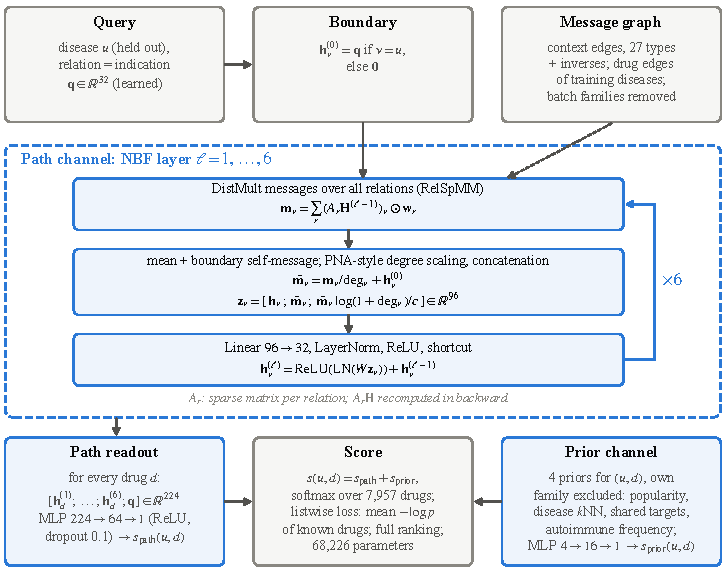
\includegraphics[width=\textwidth]{fig_architecture_tall.pdf}
\caption{\sysname architecture: six NBF layers pass DistMult messages from the query disease $u$ over a graph without the drug edges of $u$'s family; path and prior scores are summed to rank all 7,957 drugs.}
\label{fig:arch}
\end{figure}

\section{Method}
\textbf{Path channel.} For a query disease $u$, node states start from an indicator, $h^{(0)}_v=\mathbf{1}[v=u]\,q$, with a learned query vector $q$, and pass through $L=6$ layers
\begin{align}
m^{(t)}_v &= \frac{1}{\deg v}\sum_{(x,r,v)} h^{(t-1)}_x \odot w^{(t)}_r \;+\; \mathbf{1}[v=u]\,q,\label{eq:msg}\\
h^{(t)}_v &= h^{(t-1)}_v + \mathrm{ReLU}\big(\mathrm{LN}\big(W^{(t)}[h^{(t-1)}_v;\, m^{(t)}_v;\, a_v m^{(t)}_v]\big)\big),\label{eq:upd}
\end{align}
with DistMult relation vectors $w_r$ in (\ref{eq:msg}) and a PNA-style degree scaler $a_v$~\citep{corso2020pna} in (\ref{eq:upd}). An MLP over $[h^{(1)}_d;\dots;h^{(L)}_d;q]$ scores every drug $d$ in one pass (Fig.~\ref{fig:arch}). One sparse matrix per relation and a custom autograd function that recomputes products in the backward pass make memory grow with nodes, not edges.

\textbf{Prior channel and training.} A small MLP over four features adds a second score: drug popularity among training diseases, a disease-similarity $k$NN score ($k=20$, TF--IDF over disease proteins and phenotypes), shared drug-target/disease-gene count, and frequency among autoimmune training diseases, each computed with the query's family excluded. The loss is the mean negative log-softmax of each disease's known drugs over all drugs. Hyperparameters were fixed in advance, not tuned.

\textbf{Evaluation.} All drugs are ranked with \emph{filtered} ranks (other known drugs removed)~\citep{bordes2013transe}. Table~\ref{tab:metricdefs} defines the metrics. On the test split, MRR~\citep{voorhees1999trec} is \TestMrr{}; the median known-drug rank is \MedRankTest, and \RankOneShareTest\% are ranked first. AUROC is high even for popularity (\PopValidAuroc), so it is never used alone~\citep{saito2015prc}. The 68 validation diseases select the stopping epoch; 68 further \emph{test} diseases are used for neither training nor stopping. Of six non-neural baselines and three KG embeddings (TransE, DistMult, RotatE, same graph), the strongest is disease $k$NN (drugs of the 20 most similar training diseases). CIs are bootstraps over diseases~\citep{efron1993bootstrap}; a difference is significant only if the paired CI excludes zero \emph{and} a two-sided Wilcoxon test gives $p<0.05$~\citep{wilcoxon1945}.

\textbf{Reproducibility.} Data: PrimeKG (Harvard Dataverse, \url{https://doi.org/10.7910/DVN/IXA7BM}) and TxGNN's area files and code (GitHub, commit 0e0203c). Split seeds: validation 0, test 1, controls 100--102 (JSON). Model: as in Fig.~\ref{fig:arch} (dimension 32, 6 layers, dropout 0.1). Training: Adam, learning rate $5\times10^{-3}$, 8 diseases per batch, gradient clipping 1.0, $\leq$20 epochs, patience 5--6 on validation MRR (transfer runs: $\leq$60 epochs, patience 10); seeds 0--2; one NVIDIA T4 per run (5.8\,GB peak). Statistics: 1,000 bootstrap resamples (5,000 for paired tests). Code, splits, logs and number-generating scripts: \url{https://github.com/SaiYatin/Capstone_Drug_Repurposing_Project} (branch \texttt{bpp-v3}).

\section{Results}\label{sec:results}
\subsection{Aim 1: Transfer to Rare Autoimmune Diseases}
\emph{Scarce data} (Fig.~\ref{fig:transfer}). Trained only on the RA/SLE/MS families (A), \sysname reaches MRR \TrAEMrr{} on $E$, against \TrActlEMrr{} with label-matched non-autoimmune diseases (A$'$): a significant difference of \DiffTrAActlE{} (CI \DiffLoTrAActlE{} to \DiffHiTrAActlE; $p$\,\PwilTrAActlE; better on \WinsTrAActlE{} of 12), also with final checkpoints ($p$\,\PwilTrAActlELast). The targets (\TrATargetsMrr{} vs.\ \TrActlTargetsMrr; $p$\,\PwilTrAActlTargets, $n=6$) and disease $k$NN (\TrAEKnnMrr{} vs.\ \TrActlEKnnMrr) point the same way. What transfers is a drug-class prior: the A model ranks the same corticosteroids first for every target. With paths only, both stay near the floor (\TrAPathsEMrr{} vs.\ \TrActlPathsEMrr), so the advantage comes from the prior channel.

\begin{table}[tb]
\begin{minipage}[b]{0.535\textwidth}
\centering
\captionof{table}{Metrics (per disease over all 7,957 drugs, then averaged) and their value for a random ranking.}
\label{tab:metricdefs}
\scriptsize
\setlength{\tabcolsep}{2pt}
\begin{tabular}{@{}p{1.1cm}>{\raggedright\arraybackslash}p{3.8cm}r@{}}
\toprule
Metric & Meaning & Random\\
\midrule
Any@10 & share of diseases with a known drug in the top 10 & \RandExpAnyTenTest\%\\
H@$k$ & share of known drugs in the top $k$ (Hits@$k$) & $k/7957$\\
MRR & mean of $1/\text{rank}$ over known drugs (1 = all first) & $\approx$0.001\\
AUROC & chance a known drug outranks a random other drug & 0.5\\
AUPRC & area under precision--recall; rewards known drugs at the top & $\approx$0.001\\
\bottomrule
\end{tabular}
\end{minipage}\hfill
\begin{minipage}[b]{0.44\textwidth}
\centering
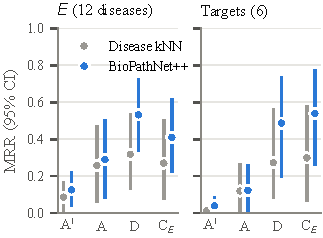
\includegraphics[width=\linewidth]{fig_transfer_curve_half.pdf}
\captionof{figure}{Aim 1: MRR on $E$ (left) and the targets (right) by training set (95\% CIs).}
\label{fig:transfer}
\end{minipage}
\end{table}
\emph{Full scale.} Training on all non-autoimmune diseases (D) reaches \TrDEMrr{} on $E$; adding the autoimmune diseases (C$_E$, \TrCESeeds{} seeds) lowers it to \TrCEEMrr{} ($p$\,\PwilTrCEDE; same validation set), and disease $k$NN drops too (\TrDEKnnMrr{} to \TrCEEKnnMrr). On the targets, removing all autoimmune diseases changes nothing (\NoautoTargetsMrr{} vs.\ \MainTargetsMrr; $p$\,\PwilMainNoautoTargets).

\subsection{Aim 2: Accuracy on Unseen Diseases}
On the selection-free test split (Table~\ref{tab:main}), a known indication is in the top 10 for \TabModelTestAnyTen\% of diseases, against \TabKnnTestAnyTen\% for disease $k$NN, \TabPopTestAnyTen\% for popularity and \RandExpAnyTenTest\% by chance. MRR is \TestMrr{} vs.\ \KnnTestMrr{} (difference \DiffTestKnn, CI \DiffLoTestKnn{} to \DiffHiTestKnn; $p$\,\PwilTestKnn). On validation the gain over $k$NN is \DiffMainKnnValid{} ($p$\,\PwilMainKnnValid). \sysname thus outperforms every baseline evaluated on the same leakage-free split; on the six targets it is ahead for \WinsMainKnnTargets{} of 6 (not significant).

\begin{table}[!htbp]
\centering
\caption{Aim 2: ranking of all 7,957 drugs (metrics: Table~\ref{tab:metricdefs}). AUROC hard/deg.: against drugs indicated for autoimmune diseases / degree-matched drugs. Test: never used for model selection; seed means (\TestSeeds{} seeds; KG embeddings \KgeRotateSeeds).}
\label{tab:main}
\scriptsize
\setlength{\tabcolsep}{3pt}
\setlength{\tabcolsep}{2pt}
\begin{tabular}{lcccccccccc}
\toprule
Method & Any@10 & H@1 & H@10 & H@50 & AUROC & AUROC & AUROC & AUPRC & MRR & Mean\\
 & & & & & & hard & deg. & & & rank\\
\midrule
\multicolumn{11}{l}{\textit{Test (68 diseases)}}\\
Random & 1\% & 0.000 & 0.005 & 0.006 & 0.453 & 0.471 & 0.500 & 0.002 & 0.001 & 4,349\\
Popularity & 19\% & 0.042 & 0.070 & 0.267 & 0.885 & 0.562 & 0.812 & 0.084 & 0.062 & 918\\
TransE & 27\% & 0.019 & 0.061 & 0.146 & 0.880 & 0.674 & 0.773 & 0.050 & 0.037 & 952\\
DistMult & 22\% & 0.025 & 0.089 & 0.193 & 0.852 & 0.638 & 0.732 & 0.060 & 0.047 & 1,175\\
RotatE & 27\% & 0.052 & 0.094 & 0.209 & 0.878 & 0.723 & 0.785 & 0.089 & 0.071 & 971\\
Disease $k$NN & 57\% & 0.347 & 0.459 & 0.583 & 0.907 & 0.721 & 0.859 & 0.429 & 0.392 & 742\\
\textbf{\sysname} & 76\% & 0.435 & 0.637 & 0.727 & 0.959 & 0.862 & 0.924 & 0.556 & 0.501 & 329\\
\midrule
\multicolumn{11}{l}{\textit{Validation (68 diseases)}}\\
Random & 1\% & 0.000 & 0.002 & 0.004 & 0.471 & 0.488 & 0.490 & 0.002 & 0.001 & 4,205\\
Popularity & 15\% & 0.034 & 0.049 & 0.188 & 0.830 & 0.476 & 0.760 & 0.069 & 0.046 & 1,355\\
Disease $k$NN & 44\% & 0.239 & 0.350 & 0.490 & 0.860 & 0.661 & 0.822 & 0.313 & 0.281 & 1,118\\
\textbf{\sysname} & 56\% & 0.353 & 0.456 & 0.601 & 0.938 & 0.799 & 0.886 & 0.424 & 0.394 & 495\\
\midrule
\multicolumn{11}{l}{\textit{Rare targets (6 diseases)}}\\
Random & 0\% & 0.000 & 0.000 & 0.000 & 0.476 & 0.488 & 0.389 & 0.002 & 0.001 & 4,165\\
Popularity & 50\% & 0.062 & 0.148 & 0.162 & 0.905 & 0.460 & 0.766 & 0.116 & 0.099 & 755\\
Disease $k$NN & 67\% & 0.243 & 0.424 & 0.725 & 0.962 & 0.778 & 0.917 & 0.407 & 0.296 & 299\\
\textbf{\sysname} & 83\% & 0.396 & 0.648 & 0.695 & 0.982 & 0.892 & 0.954 & 0.594 & 0.475 & 141\\
\bottomrule
\end{tabular}
\end{table}

\subsection{Aim 3: Contribution of Each Component}
Paths carry the signal: on validation, paths alone reach MRR \PathsValidMrr{}, tied with the full model's \MainValidMrr{} ($p$\,\PwilMainPathsValid); the prior channel alone reaches \PriorValidMrr. These are not comparable with the test MRR of \TestMrr{}: the test diseases are easier for every method ($k$NN \KnnTestMrr{} on test vs.\ \KnnValidMrr{} on validation). The prior channel does not raise the mean but cuts seed variance on the targets (sd \MainTargetsMrrSd{} vs.\ \PathsTargetsMrrSd). Self-adversarial BCE is not significantly worse than the listwise loss (\BceValidMrr{} vs.\ \MainValidMrr; $p$\,\PwilMainBceValid), and dropping tissue-expression and drug--drug edges removes \BrgEdgeCutPct\% of edges at unchanged accuracy ($p$\,\PwilMainBrgValid).

\subsection{Case Studies and Validation}
\emph{Known drugs.} Ursodeoxycholic acid ranks first for PBC in every seed; the four labeled cholinesterase inhibitors hold ranks 1--4 for MG. AIH scores near zero only because PrimeKG lists one off-label drug; the top choice, prednisolone, is standard therapy (comparator in NCT00838214).
\emph{Unlabeled candidates} (Table~\ref{tab:validation}). We searched ClinicalTrials.gov for each candidate and two reference sets (popularity top 20; 20 random drugs per target), requiring a whole-name match to a named intervention (A: phase $\geq$3, B: 2, C: 1/observational). A trial \emph{tests} the drug only if its title names it or the drug is in some but not all arms (not as background therapy). Of the model's candidates, \ValTrialTestedModel\% have such a trial (\ValGradeATested{} at phase $\geq$3), against \ValTrialTestedPop\% (popularity) and \ValTrialTestedRand\% (random); e.g.\ amifampridine for MG (NCT03304054) and ciprofloxacin for Crohn (NCT00609973), checked by hand. A trial is no proof of benefit: amifampridine helped in MuSK-antibody MG~\citep{bonanno2018amifampridine} but not in AChR-antibody MG~\citep{remijn2026amifampridine}. Ustekinumab--Crohn is unlabeled only because PrimeKG misses its 2016 approval. AI-assisted PubMed title labels were each re-checked against the abstract. PubMed shows benefit for \ValLitSupModel\% of candidates (popularity \ValLitSupPop\%, random \ValLitSupRand\%) and harm or no benefit for \ValLitAgainstModel\% (popularity \ValLitAgainstPop\%): three corticosteroid pairs and N-acetylcysteine for SSc; popularity's are mostly antibiotics that can worsen MG or induce hepatitis.

\begin{table}[tb]
\centering
\caption{Evidence for unlabeled top-20 candidates (Ours $n$=\ValNovelN; others $n$=120).}
\label{tab:validation}
\scriptsize
\setlength{\tabcolsep}{3pt}
\begin{tabular}{lccc@{\hspace{14pt}}lccc}
\toprule
Clinical trials & Ours & Pop. & Rand. & Literature and targets & Ours & Pop. & Rand.\\
\midrule
Trial names drug, A--C & 17\% & 14\% & 0\% & PubMed co-mention & 63\% & 72\% & 18\%\\
Trial names drug, A--B & 15\% & 12\% & 0\% & PubMed: benefit & 15\% & 10\% & 0\%\\
Trial tests drug, A--C & 13\% & 8\% & 0\% & PubMed: harm/no benefit & 5\% & 12\% & 0\%\\
Trial tests drug, A--B & 12\% & 8\% & 0\% & Drug targets a disease gene & 17\% & 16\% & 3\%\\
\bottomrule
\end{tabular}
\end{table}
\emph{Temporal check.} Six drugs approved after the PrimeKG snapshot (risankizumab, upadacitinib, guselkumab for Crohn; ravulizumab, rozanolixizumab for MG; elafibranor for PBC) rank at a median of \TempPostMedRank{} of 7,957 (\TempPostBetter{} of 6 above chance; $p$\,\TempPostP).
\emph{Explanations and bias.} Gradient-based path extraction~\citep{zhu2021nbfnet} shows that amifampridine reaches MG through its indication for the related Lambert--Eaton syndrome and exposes weak links such as ciprofloxacin reaching Crohn through ``mouth disease''. Corticosteroids fill \ValSteroidShare\% and antibacterials \ValAntibioticShare\% of top-20 slots, so the lists need expert filtering.

\section{Discussion and Limitations}
BioPathNet reports MRR of about 0.2--0.8 on TxGNN's disease areas~\citep{hu2026biopathnet}, but on other splits; we therefore ran TxGNN's own code on its autoimmune split, training our model only on edges TxGNN also trains on (\TxhSeedsTx{} seeds, \TxhN{} diseases). Ranking all drugs, \sysname is significantly better (MRR \TxhOursMrr{} vs.\ \TxhTxMrr, $p$\,\TxhPwilFullMrr): only \TxhTxIndShare\% of TxGNN's top-100 drugs have any indication, against \TxhOursIndShare\% for ours. Ranking only drugs with indications, as TxGNN does, nothing is significant (Recall@100 \TxhOursRecall{} vs.\ \TxhTxRecall; AUROC \TxhOursAuroc{} vs.\ \TxhTxAuroc). BioPathNet was not re-run.
Limitations: (i) the targets have 1--24 labeled drugs, so their metrics are noisy lower bounds (AIH); (ii) validation diseases also choose the stopping epoch (\SelGapMainMin--\SelGapMainMax{} MRR of optimism), which the test split avoids; (iii) $E$ has 12 diseases, and 11-disease models are seed-unstable; (iv) no clinician has reviewed the literature labels.

\section{Conclusion}
Path-based zero-shot transfer works for rare autoimmune diseases the model never sees: related autoimmune diseases are the best source when data is scarce, the broad pharmacological graph at full scale. \sysname outperforms every baseline evaluated on the same leakage-free split, recovers established therapies, and ranks later-approved drugs high but not significantly above chance. Paths drive accuracy; the prior channel adds stability.

\paragraph{Acknowledgments.} Generative AI tools assisted with code, analysis and language editing; the authors verified all results against the released run logs.

\bibliographystyle{spmpsci}
\bibliography{references}

\end{document}
